%&../settings/preamble.main

% NOTE per controllare dove sfori la pagina
% \setlength\overfullrule{5pt}

\ifsubfile
\pagestyle{plain}
\setcounter{chapter}{17}

% arara: pdflatex: { options: ["--output-directory=../build"], draft: yes, synctex: no }
% arara: pdflatex: { options: ["--output-directory=../build"], synctex: no }
\begin{document}
\fi
\chapter[Problemi intrattabili e Teoria dell'NP-completezza]{Problemi intrattabili\\Teoria dell'NP-completezza}

\section*{Introduzione}

Con l'eccezione della sezione su backtrack, finora abbiamo considerato solo problemi con soluzioni in tempo polinomoniale.
Il tempo di esecuzione per queste soluzioni è \(\Omicron(n^k)\) per qualche \(k\).

Esistono problemi che per essere risolti hanno bisogno di un tempo almeno esponenziale (che indicheremo con \EXPTIME).
Valutare una posizione di scacchi, dama, go; Oppure risolvere il problema delle Torri di Hanoi sono esempi di problemi con tempo almeno esponenziale.
Esistono inoltre problemi per i quali non esiste alcuna soluzione.
Come ad esempio il problema della terminazione (\foreign{halting problem}).

In questa lezione discuteremo di una classe di problemi per cui non è chiaro se esista un algoritmo polinomoniale oppure no; questi problemi sono tutti nella stessa barca: potrebbero essere tutti risolti in tempo polinomoniale, oppure nessuno di essi.

I problemi per il millennio (\foreign{Millennium problems}) sono sette problemi posti all'attenzione dei matematici dell'Istituto Clay.
Per chi risolve uno di questi problemi c'è in palio un milione di dollari.
Ad oggi, solo un problema è stato risolto (la Congettura di Poincarè).

\paragraph{Problema astratto}
Un problema astratto è una relazione binaria \(R \subseteq I \times S\) tra un insieme \(I\) di istanze del problema e un insieme \(S\) di soluzioni.

Ad esempio prendiamo in considerazione il problema del cammino minimo (\shortestPath).
Una sua istanza è una quadrupla (\(V\), \(E\), \(u\), \(v\)), e una sua soluzione è una sequenza ordinata di vertici \(v_1, \dots, v_k\).

\begin{note}
Possono esistere più soluzioni associate alla stessa istanza.
\end{note}

\subsection*{Tipologie di problemi}

Esistono diverse tipologie di problemi: problemi di \textbf{ottimizzazione}, di \textbf{ricerca} o di \textbf{decisione}.

Nei \textbf{problemi di ottimizzazione} data un'istanza, dobbiamo trovare la \enquote{migliore} soluzione secondo criteri specifici.
Ad esempio nel problema del cammino minimo dato un grafo \(G\) e due nodi \(u\), \(v\), dobbiamo trovare il cammino più breve fra essi.

Nei \textbf{problemi di ricerca} data un'istanza, dobbiamo trovare una possibile soluzione fra quelle esistenti.
Ad esempio nel problema della ricerca di un cammino dato un grafo \(G\) e due nodi \(u\), \(v\), dobbiamo trovare un cammino fra essi.

Nei \textbf{problemi di decisione} data un'istanza, cerchiamo semplicemente di verificare se soddisfa o meno una data proprietà.
La relazione in questo caso è una funzione \(R: I \to \{0,1\}\).
Prendiamo di nuovo in considerazione il problema del percorso minimo ma stavolta ci poniamo una domanda.
Dati un grafo \(G\), due nodi \(u\), \(v\) e un valore \(k\), esiste un cammino tra \(u\) e \(v\) di lunghezza minore o uguale a \(k\)?

\paragraph{Equivalenza fra problemi di ottimizzazione e decisione}
In quanto la versione decisionale dei problemi è più semplice da trattare matematicamente, ragioneremo in termini di problemi di decisione e non di ottimizzazione.

Difatti se posso risolvere efficientemente la versione di ottimizzazione, allora posso risolvere efficientemente la versione di decisione.
\'{E} vero anche l'opposto.
Ossia, se \emph{non} posso risolvere efficientemente la versione di decisione, allora \emph{non} posso risolvere efficientemente la versione di ottimizzazione.

Ad esempio, riconducendoci sempre al problema del cammino più breve, se conosco il cammino più breve, posso rispondere alla domanda decisionale per qualunque valore di \(k\).

\section{Riduzioni}

\subsection{Riduzione polinomiale}

Dati due problemi decisionali \(R_1 \subseteq I_1 \times \{0,1\}\) e \(R_2 \subseteq I_2 \times \{0,1\}\), \(R_1\) è riducibile polinomialmente a \(R_2\) (si scrive matematicamente \(R_1 \leqslant_p R_2\)) se esiste una funzione \(f: I_1 \to I_2\) con le seguenti proprietà:
\begin{itemize}
    \item \(f\) è calcolabile in tempo polinomiale;
    \item per ogni istanza \(x\) del problema \(R_1\) e ogni soluzione \(s \in \{0,1\}\), \((x,s) \in R_1 \Leftrightarrow (f(x), s) \in R_2\).
\end{itemize}

\begin{figure}[H]\centering
	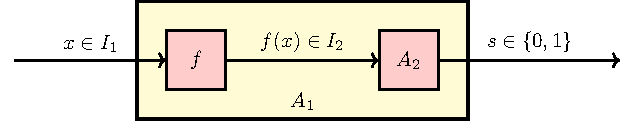
\includegraphics{riduzione}
\end{figure}

\begin{minipage}[c]{.7\textwidth}
\subsection{Colorazione di grafi}

Dati un grafo non orientato \(G = (V,E)\) e un insieme di colori \(C\), una colorazione dei vertici è un assegnamento \(f: V \to C\) che \enquote{colora} ogni nodo con uno dei valori in \(C\), tale per cui nessuna coppia di nodi adiacenti ha lo stesso colore.

Possiamo formulare il problema sia sotto forma di problema di ottimizzazione, che decisionale.
Nella forma decisionale dobbiamo determinare \emph{se esiste}, dato un grafo non orientato \(G = (V,E)\) e un valore \(k\), una colorazione \(G\) con \(k\) colori; mentre nella forma di ottimizzazione dobbiamo restituire la colorazione che necessita del numero minimo di colori.
\end{minipage}%
\begin{minipage}[c]{.3\textwidth}
\begin{figure}[H]\centering
	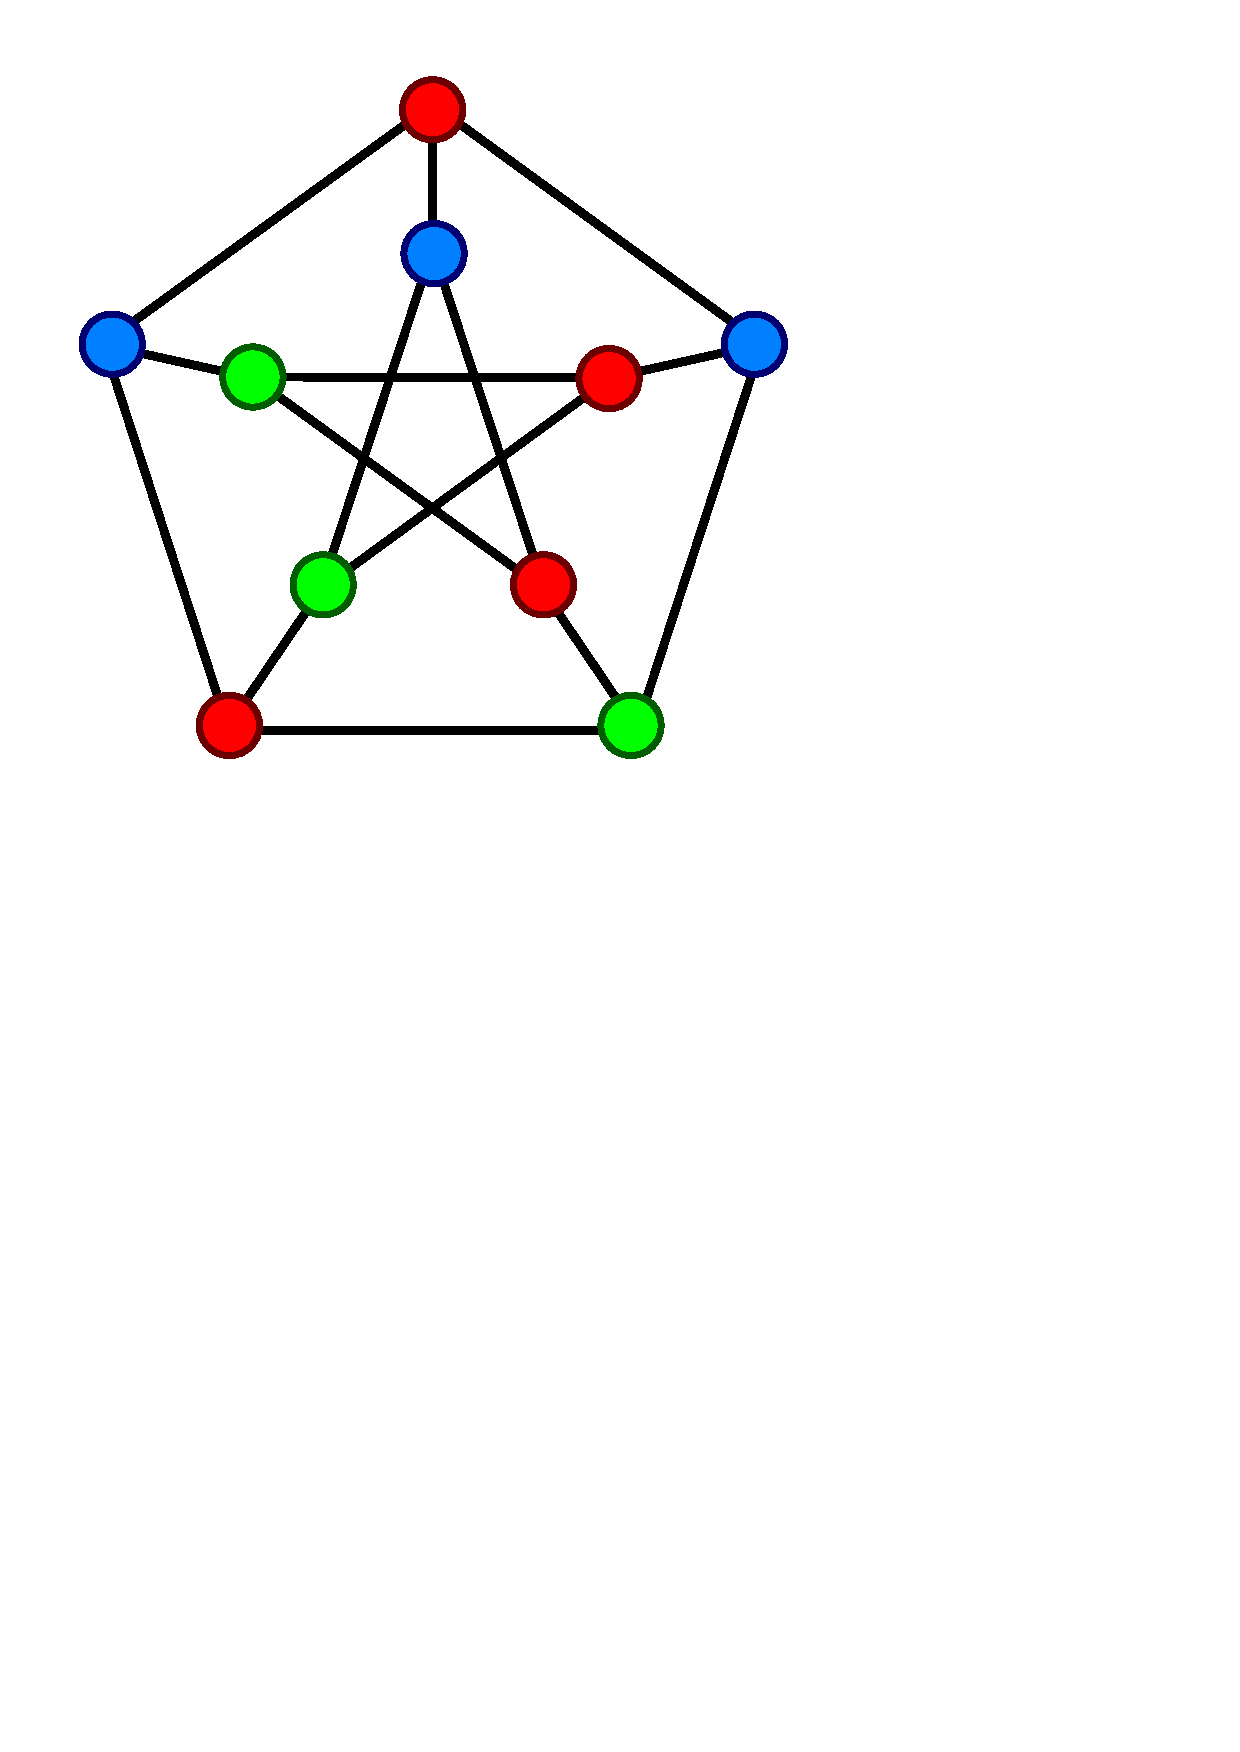
\includegraphics[width=0.8\textwidth]{coloring}
\end{figure}
\end{minipage}

\subsection{Sudoku}

Il problema generale del Sudoku richiede di inserire dei numeri fra 1 e \(n^2\) in una matrice di \(n^2 \times n^2\) elementi suddivisa in \(n \times n\) sottomatrici di dimensione \(n \times n\), in modo tale che nessun numero compaia più di una volta in ogni riga, colonna e sottomatrice.

Esistono due versioni di questo problema, entrambe espresse in forma decisionale.

Le prima versione è quella classica: data una matrice \(n^2 \times n^2\) elementi, determinare se esiste un modo per assegnare i numeri in modo da rispettare le regole del Sudoku.

Mentre nella seconda abbiamo qualche numero già presente: data una matrice \(n^2 \times n^2\) elementi con alcuni numeri già presenti nella matrice, determinare se esiste un modo per assegnare i numeri in modo da rispettare le regole del Sudoku.

\subsubsection*{Riduzione da problema particolare a problema generale}

\paragraph{Riduzione in tempo polinomiale}
\(V = \{(x,y): 1 \leqslant x \leqslant n^2, 1 \leqslant y \leqslant n^2\}\)

\([(x,y),(x',y')] \in E \Leftrightarrow\)
\begin{itemize}
    \item \(x = x'\); oppure,
    \item \(y = y'\); oppure,
    \item \((\ceil{x/n} = \ceil{x'/n}) \land ((\ceil{y/n} = \ceil{y'/n}))\)
\end{itemize}
\(C = \{1, \dots, n\}\).

Se abbiamo una soluzione per la colorazione, allora abbiamo una soluzione algoritmica per il Sudoku. Scriveremo quindi che \(\sudokuProblem \leqslant_p \graphColoring\).

Troviamo diverse applicazioni. Come ad esempio nell'assegnamento delle radio frequenze in un insieme di torri cellulari. O nell'allocazione degli esami universitari.

\begin{minipage}[c]{.7\textwidth}
\subsection{Insieme indipendente}

Sia dato un grafo non orientato \(G = (V,E)\); un insieme \(S \subseteq V\) è un insieme indipendente se e solo se nessun arco unisce due nodi in \(S\).
Matematicamente scriveremo
\[
    \forall (x,y) \in E : x \not\in S \lor y \not\in S
\]
Possiamo formulare il problema sia sotto forma di problema di ottimizzazione, che decisionale.
Nella forma decisionale dobbiamo determinare \emph{se esiste}, dato un grafo non orientato \(G = (V,E)\) e un valore \(k\), un insieme indipendente di dimensione \(k\); mentre nella forma di ottimizzazione dobbiamo restituire il più grande insieme indipendente presente nel grafo.
\end{minipage}%
\begin{minipage}[c]{.3\textwidth}
\begin{figure}[H]\centering
	\includegraphics[page=2, width=0.7\textwidth]{independent}
\end{figure}
\end{minipage}

\paragraph{Packing problem}
Questo è un esempio di packing problem, un problema in cui si cerca di selezionare il maggior numero di oggetti, la cui scelta è però soggetta a vincoli di esclusione.
I problema dello zaino ne è l'esempio prìncipe.

\begin{minipage}[c]{.7\textwidth}
\subsection{Copertura di vertici}

Dato un grafo non orientato \(G = (V,E)\), un insieme \(S \subseteq V\) è una copertura di vertici se e solo se ogni arco ha almeno un estremo in \(S\).
Matematicamente scriveremo
\[
    \forall (x,y) \in E : x \in S \lor y \in S
\]
Possiamo formulare il problema sia sotto forma di problema di ottimizzazione, che decisionale.
Nella forma decisionale dobbiamo determinare \emph{se esiste}, dato un grafo non orientato \(G = (V,E)\) e un valore \(k\), una copertura di vertici di dimensione al massimo \(k\); mentre nella forma di ottimizzazione dobbiamo restituire la copertura dei vertici di dimensione minima.
\end{minipage}%
\begin{minipage}[c]{.3\textwidth}
\begin{figure}[H]\centering
	\includegraphics[page=2, width=0.7\textwidth]{cover}
\end{figure}
\end{minipage}

\paragraph{Covering problem}
Questo è un esempio di covering problem, un problema in cui si cerca di ottenere il più piccolo insieme in grado di coprire un insieme arbitrario di oggetti con il più piccolo sottoinsieme di questi oggetti.

\subsection{Riduzione per problemi duali}

% \subsubsection{Da insieme indipendente a copertura di vertici}
\subsubsection{Se \(S \subseteq V\) è un insieme indipendente, allora \(V - S\) è una copertura di vertici}

Se \(S\) è un insieme indipendente:
\begin{itemize}
    \item ogni arco \((x,y)\) non può avere entrambi gli estremi in \(S\);
    \item quindi almeno uno dei due deve essere in \(V-S\).
\end{itemize}
\begin{figure}[H]\centering
	\includegraphics[page=3, width=0.4\textwidth]{independent}
\end{figure}

% \subsubsection{Da copertura di vertici a insieme indipendente}
\subsubsection{Se \(V - S\) è una copertura di vertici, allora \(S \subseteq V\) è un insieme indipendente}

Supponiamo per assurdo che \(S\) non sia un insieme indipendente:
\begin{itemize}
    \item allora esiste un arco \((x,y)\) che unisce due nodi in \(S\);
    \item nessuno dei due estremi sta in \(V-S\);
    \item questo implica che \(V-S\) non è una copertura di vertici, il che è assurdo.
\end{itemize}
\begin{figure}[H]\centering
	\includegraphics[page=3, width=0.4\textwidth]{cover}
\end{figure}

\subsection{Equivalenza dei problemi}

Se il problema della copertura di vertici è riducibile al problema dell'insieme indipendente.
\[
    \vertexCover \leqslant_p \indipendentSet
\]
E il problema dell'insieme indipendente è riducibile al problema della copertura di vertici.
\[
    \indipendentSet \leqslant_p \vertexCover
\]
Abbiamo dimostrato che i due problemi sono equivalenti.

\subsection{Soddisfacibilità di formule booleane}

Data un'espressione in forma normale congiuntiva, il problema della soddisfacibilità consiste nel decidere se esiste una assegnazione di valori di verità alle variabili che rende l'espressione vera.

Ad esempio se prendiamo l'espressione \((x \lor \bar{y} \lor z) \land (\bar{x} \lor w) \land y\) e assegniamo ad ogni variabile il valore di verità \True, allora possiamo riscrivere l'espressione come \((\True \lor \False \lor \False) \land (\False \lor \True) \land \True\), semplificando ulteriormente otteniamo \(\True \land \True \land \True\), ed infine \(\True\).
Possiamo dedurne quindi che la formula booleana iniziale è soddisfacibile, in quanto esiste almeno un'interpretazione delle variabili che la rende vera.

Riduciamo il problema generale ad una forma che include solo tre letterali.
Chiameremo questo problema 3-\sat.
Data una espressione in forma normale congiuntiva in cui le clausole hanno esattamente 3 letterali, il problema della soddisfacibilità consiste nel decidere se esiste una assegnazione di valori di verità alle variabili che rende l'espressione vera.

Vogliamo dimostrare che il problema 3-\sat è riducibile polinomialmente a quello dell'insieme indipendente. Ossia
\[
    {\treeSat} \leqslant_p \indipendentSet
\]

\subsubsection*{Riduzione tramite \enquote{gadget}}

Data una formula \treeSat, costruiamo un grafo nel modo seguente:
\begin{itemize}
    \item per ogni clausola, aggiungiamo un terzetto di nodi, collegati fra di loro da archi;
    \item per ogni letterale che compare in modo normale e in modo negato, aggiungere un arco fra di essi (che chiameremo \emph{arco di conflitto}).
\end{itemize}
\begin{figure}[H]\centering
    \includegraphics[page=2, width=0.8\textwidth]{gadget}
    \caption[Gadgets]{La formula {\treeSat} è soddisfacibile se e solo è possibile trovare un insieme indipendente di dimensione esattamente \(k\).}
\end{figure}

\subsubsection*{Riduzione da problema particolare a problema generale}

Ovviamente il problema di soddisfacibilità delle formule booleane con sole tre variabili è riducibile polinomialmente al problema più generale.
Scriviamo quindi che \(\treeSat \leqslant_p \sat\).

Possiamo dimostrare l'inverso? Ossia che \(\sat \leqslant_p \treeSat\)?

\'{E} possibile trasformare una formula {\sat} in una formula {\treeSat} usando due semplici trucchi:
\begin{itemize}
    \item se la clausola è più lunga di tre elementi, si introduce una nuova variabile e si divide la clausola in due:
    \[
        (a \lor b \lor c \lor d) \equiv (a \lor b \lor z) \land (\bar{z} \lor c \lor d)
    \]
    \item se la clausola è più corta di tre elementi, si fa \enquote{\foreign{padding}}:
    \[
        (a \lor b) \equiv (a \lor a \lor b)
    \]
\end{itemize}

\subsection{Proprietà transitiva della riduzione polinomiale}

\'{E} facile intuire che la nozione di riducibilità polinomiale gode della proprietà transitiva.
\[
    \sat \leqslant_p \indipendentSet \leqslant_p \vertexCover
\]

\section{Classi \PTIME, \PSPACE}

\paragraph{Algoritmo}
Dati un problema di decisione \(R\) e un algoritmo \(A\) (scritto in un modello di calcolo Turing-equivalente) che lavora in tempo \(f_t(n)\) e spazio \(f_s(n)\), diciamo che A risolve \(R\) se \(A\) restituisce \(s\) su un'istanza \(x\) se e solo se \((x,s) \in R\).

\paragraph{Classi di complessità}
Data una qualunque funzione \(f(n)\), chiamiamo:
\begin{itemize}
    \item \(\TIME(f(n))\) l'insieme dei problemi decisionali risolvibili da un algoritmo che lavora in tempo \(\Omicron(f(n))\);
    \item \(\SPACE(f(n))\) gli insiemi dei problemi decisionali risolvibili da un algoritmo che lavora \mbox{in spazio \(\Omicron(f(n))\)}.
\end{itemize}

% \paragraph{Classe \PTIME}
La classe {\PTIME} è la classe dei problemi decisionali risolvibili in tempo polinomiale nella dimensione \(n\) dell'istanza di ingresso:
\[
    \PTIME = \bigcup_{c=0}^{\infty} \TIME(n^c)
\]

% \paragraph{Classe \PSPACE}
La classe {\PSPACE} è la classe dei problemi decisionali risolvibili in spazio polinomiale nella dimensione \(n\) dell'istanza di ingresso:
\[
    \PSPACE = \bigcup_{c=0}^{\infty} \SPACE(n^c)
\]

\begin{note}
\(\PTIME \subseteq \PSPACE\).
\end{note}

\section{Classe \NP}

\subsection{Certificato}

Dato un problema decisionale \(R\) e un'istanza di input \(x\) tale che \((x, \True) \in R\), un certificato è un insieme di informazioni che permette di provare che \((x, \True) \in R\).

Un'assegnamento di verità alle variabili della formula è un certificato per il problema di soddisfacibilità delle formule booleane.
Un'associazione nodo-colore \(f: V \to \{1, \dots, k\}\) è un certificato per il problema di colorazione dei grafi.
Un sottoinsieme di \(V\) di \(k\) elementi è un certificato per il problema degli insiemi indipendenti.
Tutti questi \enquote{certificati} hanno dimensione polinomiale nella dimensione dell'input.

I certificati possono essere verificati in tempo polinomiale:
\begin{itemize}
    \item in {\sat} si calcola il valore di verità della formula a partire dall'assegnamento di verità delle variabili in tempo \(\Omicron(n)\);
    \item in {\graphColoring} si verifica che nodi adiacenti non abbiano lo stesso colore in tempo \(\Omicron(m+n)\);
    \item In {\indipendentSet} si verifica che nodi in \(S\) non abbiano nodi adiacenti in \(V-S\) \mbox{in tempo \(\Omicron(m+n)\)}.
\end{itemize}

\begin{note}
La classe {\NP} è l'insieme di tutti i problemi che ammettono un certificato verificabile in tempo polinomiale.
\end{note}

\paragraph{Certificati non polinomiali}
Esistono dei certificati che non possono essere verificati in tempo polinomiale.
Ad esempio il problema \foreign{Quantified Boolean Formula (QBF)} è una generalizzazione del problema {\sat} nel quale ad ogni variabile possono essere applicati quantificatori universali ed esistenziali.
Un esempio è la formula \(\forall x \exists y \exists z ((x \lor z) \land y)\).
Si ritiene che un certificato del genere non esista.

\subsection{Definizione basata su non determinismo}

{\NP} è l'insieme di problemi decisionali che possono essere risolti da una Macchina di Turing non deterministica in tempo polinomiale.

In maniera \emph{molto} informale: dato uno stato ed un elemento di input, una macchina non deterministica può andare in un insieme finito di altri stati.
Esistono due interpretazioni per la macchina non deterministica.
Può essere una macchina che \enquote{azzecca} sempre la scelta giusta, oppure può essere una macchina non deterministica che si divide in un insieme finito di copie, una per scelta possibile.

Prendiamo ad esempio il problema {\sat} con quattro variabili.

\begin{figure}[H]\centering
    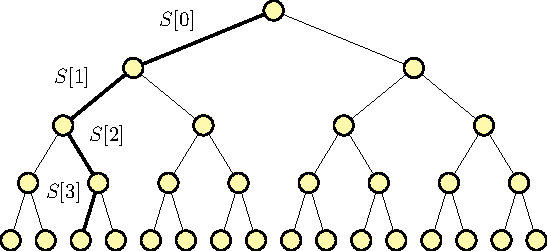
\includegraphics[width=0.8\textwidth]{branchAndBound-1}
\end{figure}

\subsection{Relazioni fra problemi}

\begin{lemma}
Se \(R_1 \leqslant_p R_2\) e \(R_2 \in \PTIME\), allora anche \(R_1\) è contenuto in \(\PTIME\).
\end{lemma}

\begin{proof}
Sia \(T_f(n) = \Omicron(n^{k_f})\) il tempo necessario per trasformare un input di \(R_1\), in input di \(R_2\), tramite una funzione \(f\).
Sia \(T_2(n) = \Omicron(n^{k_2})\) il tempo necessario per risolvere \(R_2\).
Qual è la complessità di \(R_1\)?

La funzione \(f\) può prendere un input di dimensione \(n\) e trasformarlo in un input di dimensione \(\Omicron(n^{k_f})\) per \(R_2\).
Il tempo per risolvere \(R_1\) sarà quindi \(T_1(n) = \Omicron(n^{k_f} n^{k_2})\).

Possiamo dedurre che \(T_1(n)\) è polinomiale.
\end{proof}

\section{Problemi \NP-completi}

Introduciamo alcune definizioni.

\paragraph{Problema {\NP}-arduo ({\NP}-hard)}
Un problema decisionale \(R\) si dice {\NP}-arduo se ogni problema \(Q \in \NP\) è riducibile polinomialmente a \(R\) (\(Q \leqslant_p R\)).

\paragraph{Problema {\NP}-completo ({\NP}-complete)}
Un problema decisionale \(R\) si dice {\NP}-completo se appartiene alla classe {\NP} ed è {\NP}-arduo.

\begin{note}
Se un qualunque problema decisionale {\NP}-completo appartenesse a {\PTIME}, allora risulterebbe \(\PTIME = \NP\).
\end{note}

\begin{figure}[H]\centering
    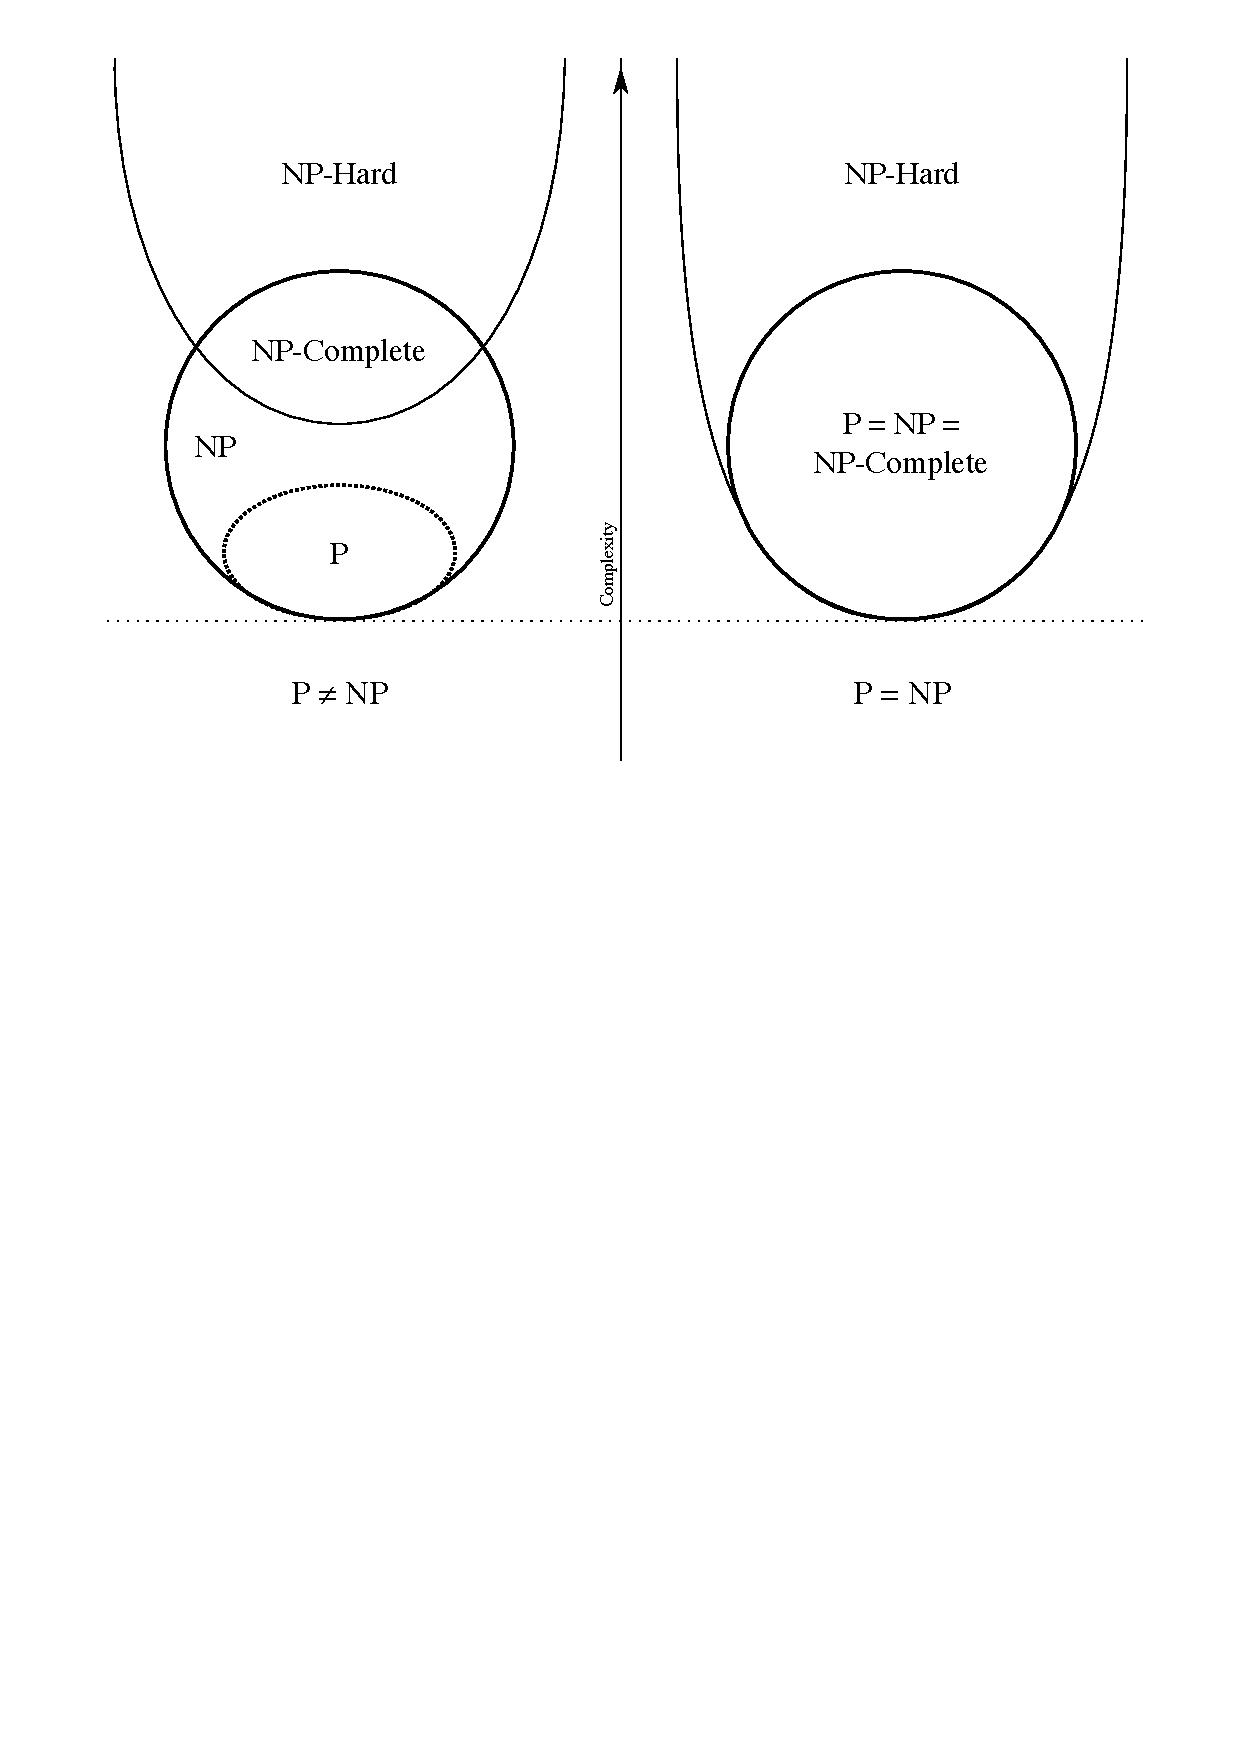
\includegraphics[width=0.8\textwidth]{pnp}
\end{figure}

Dimostrare che un problema è contenuto in {\NP} è semplice.
Dimostrare che un problema è {\NP}-completo richiede una dimostrazione difficile, apparentemente impossibile: tutti i problemi in {\NP} sono riducibili polinomialmente a tale problema, anche quelli che non conosciamo!

Nel 1973 Leonid Levin ha dimostrato in maniera indipendente il seguente teorema.
\begin{theorem*}[Teorema di Cook-Levin]
{\sat} è {\NP}-completo.
\end{theorem*}
La dimostrazione del Teorema è complessa, è basata sugli stati della macchina di Turing.

\subsubsection*{Problemi introdotti oggi}

Partendo dalle riduzioni viste oggi e utilizzando il Teorema di Cook-Levin, otteniamo:
\[
    {\sat} \leqslant_p {\treeSat} \leqslant_p {\indipendentSet} \leqslant_p {\vertexCover} \leqslant_p {\sat}
\]

In altre parole, {\treeSat}, {\indipendentSet}, {\vertexCover} sono {\NP}-completi.

In \enquote{\foreign{Reducibility Among Combinatorial Problems}} Richard Karp ha stilato una lista di 21 problemi {\NP}-completi.

\subsubsection*{I 21 problemi {\NP}-completi di Karp}

\begin{figure}[H]\centering
    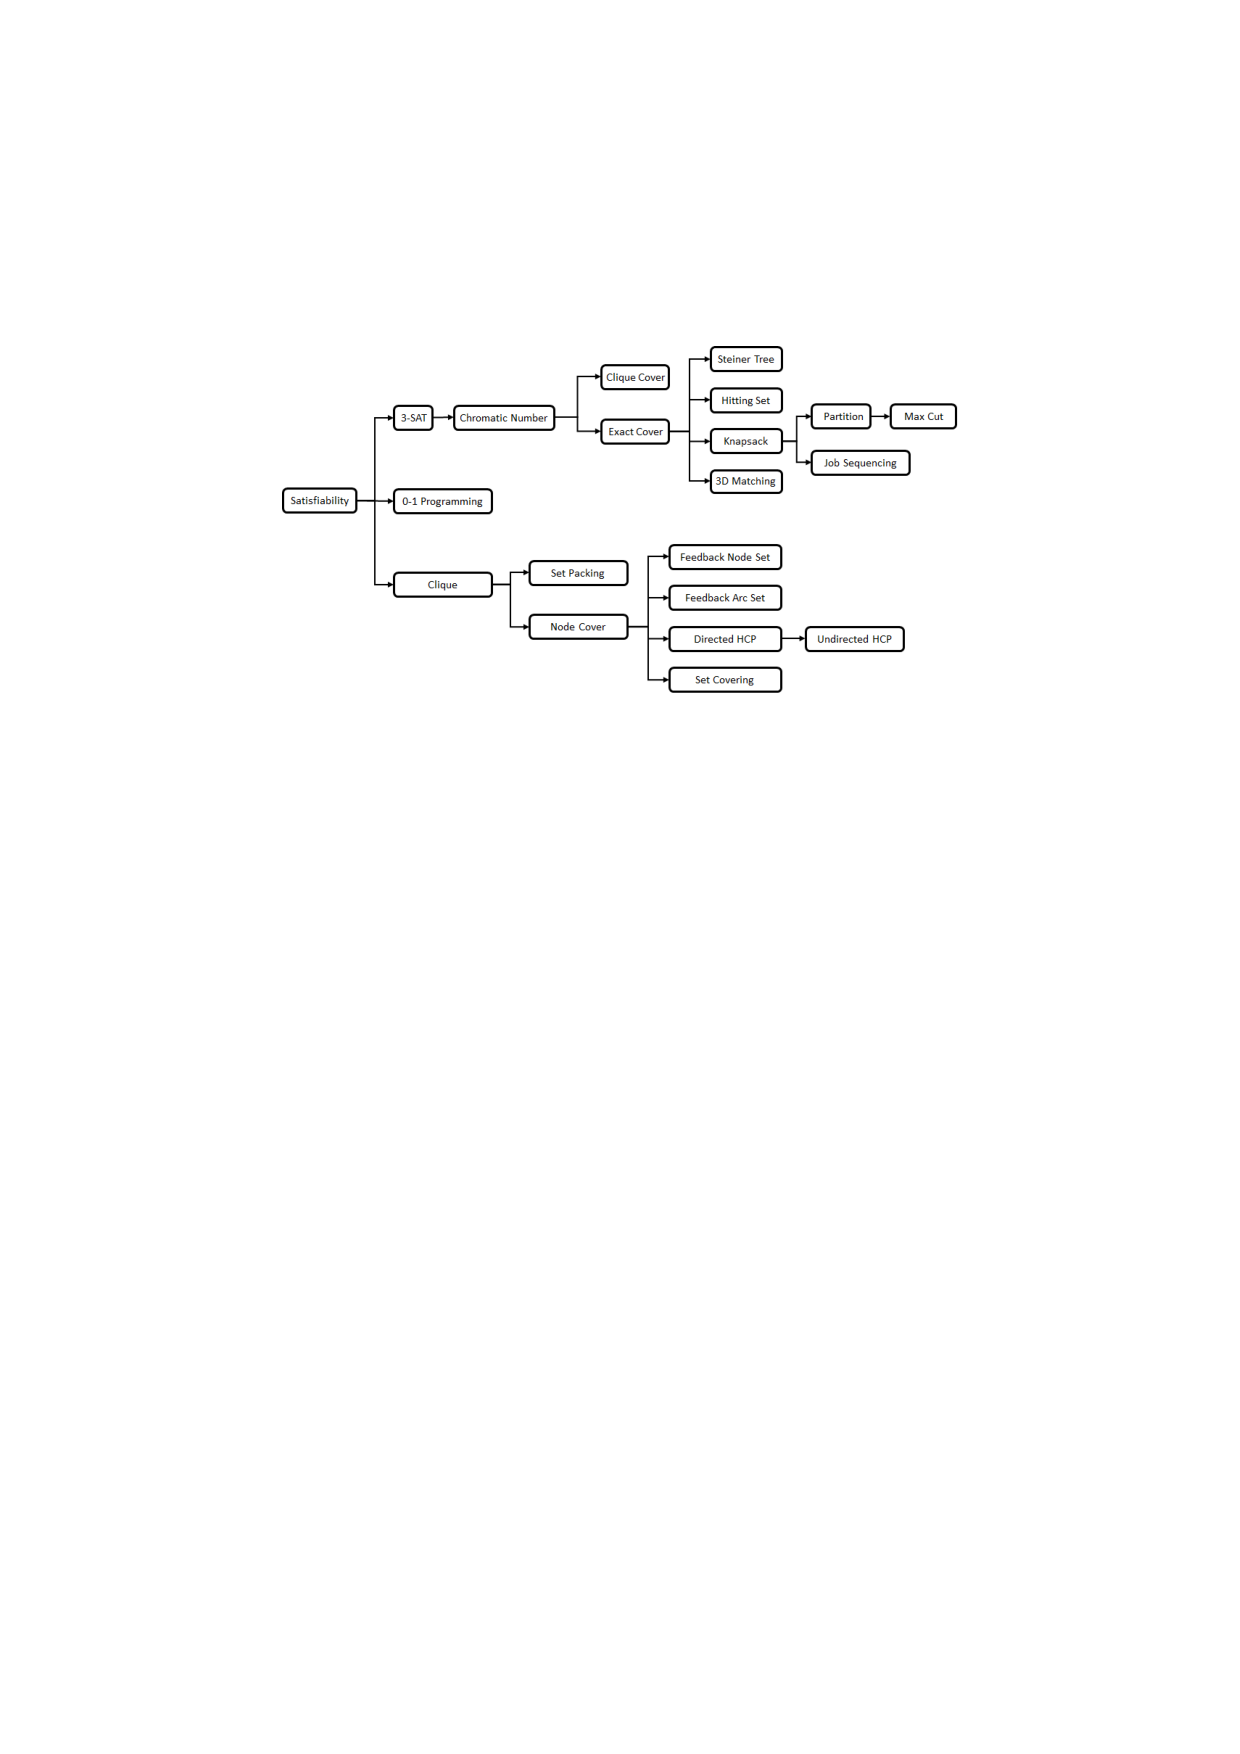
\includegraphics[width=0.8\textwidth]{karp-problems}
\end{figure}

\subsection{Problemi {\NP}-Completi \enquote{Classici}}

\begin{minipage}[c]{.7\textwidth}
\subsubsection*{Cricca (\cliqueProblem)}

Dati un grafo non orientato ed un intero \(k\), esiste un sottoinsieme di almeno \(k\) nodi tutti mutualmente adiacenti?

Questo problema trova applicazioni in bioinformatica, ingegneria elettronica e chimica.
\end{minipage}%
\begin{minipage}[c]{.3\textwidth}
\begin{figure}[H]\centering
    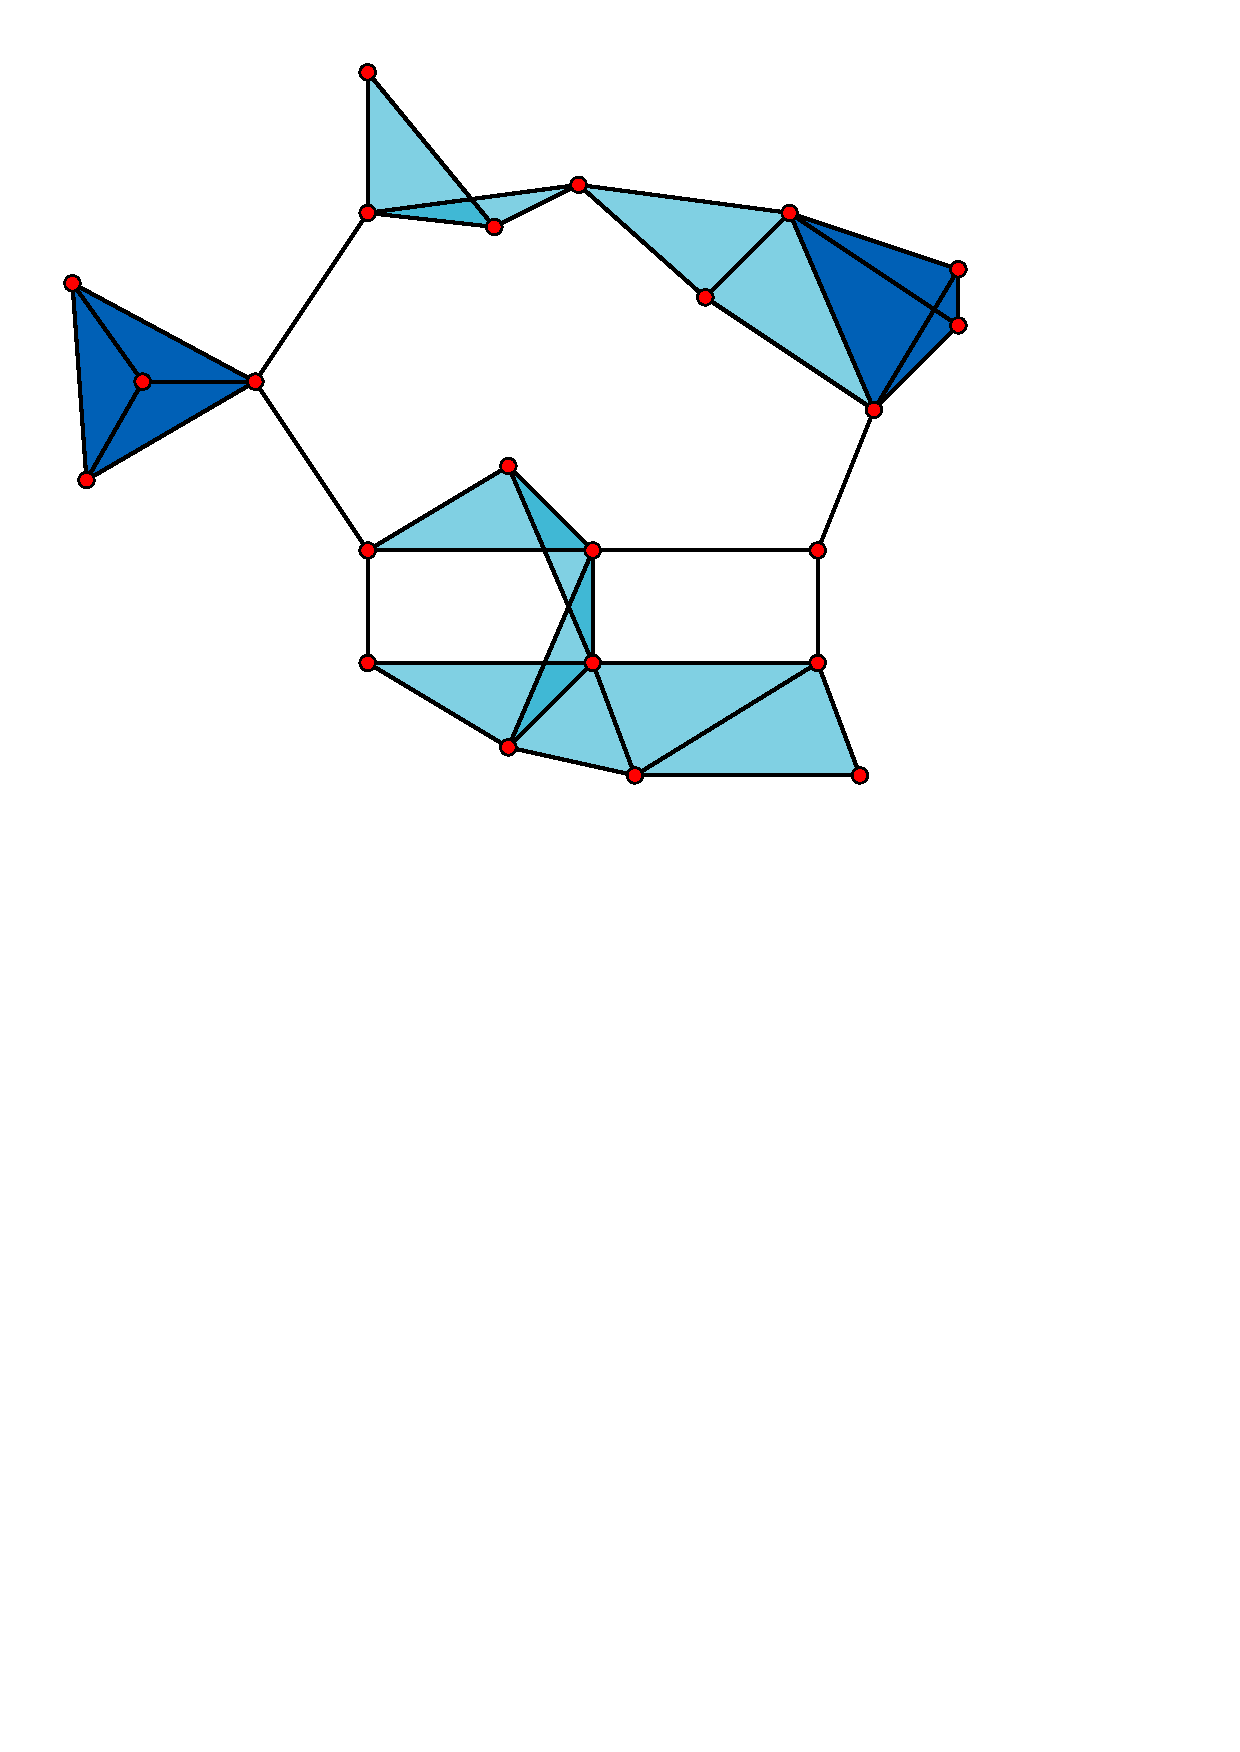
\includegraphics[width=0.8\textwidth]{clique}
\end{figure}
\end{minipage}

\begin{minipage}[c]{.3\textwidth}
\begin{figure}[H]\centering
    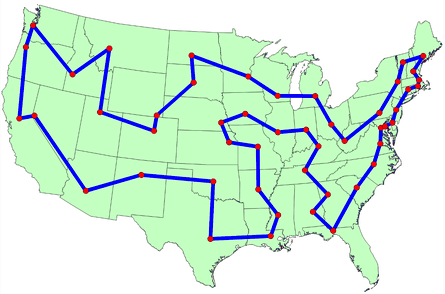
\includegraphics[width=0.8\textwidth]{tsp}
\end{figure}
\end{minipage}%
\begin{minipage}[c]{.7\textwidth}
\subsubsection*{Commesso viaggiatore (\foreign{Traveling salesperson}, {\tsp})}

Date \(n\) città, le distanze tra esse, ed un intero \(k\), è possibile partire da una città attraversare ogni città esattamente una volta tornando alla città di partenza, percorrendo una distanza non superiore a \(k\)?
\end{minipage}

\subsubsection*{Programmazione lineare \texttt{0/1}}

Data una matrice \(A\) di elementi interi e di dimensione \(m \times n\), ed un vettore \(b\) di \(m\) elementi interi, esiste un vettore \(x\) di \(n\) elementi \texttt{0/1} tale che \(Ax \leqslant b\)?

Ad esempio
\[\begin{WithArrows}[displaystyle, format=cccc]
x_1& + x_2 &+ x_3 + x_4 &\geqslant 2\\
x_1& - x_2 &- x_3 + x_4 &\geqslant 0\\
x_1&       &+ x_3 + x_4 &\geqslant 1
\end{WithArrows}\]
Il sistema è verificato per \(x_1 = x_2 = 1\) ed \(x_3 = x_4 = 0\).

\subsubsection*{Copertura esatta di insiemi}

Dato un insieme \(X\) e una collezione \(\mathcal{Y} = \{Y_1, \dots, Y_n\}\) di sottoinsiemi di \(X\), esiste una sottocollezione \(\mathcal{Z} \subseteq \mathcal{Y}\) che partizioni \(X\)?

Supponiamo che ad esempio l'insieme \(X\) sia \(\{ 1,2,3,4,5,6,7 \}\) e la collezione \(\mathcal{Y} = \{ A,B,C,D,E,F \}\) sia così composta:
\begin{align*}
A &= \{ 1,4,7 \} & B &= \{ 1,4 \} & C &= \{ 4,5,7 \} & D &= \{ 3,5,6 \} & E &= \{ 2,3,6,7 \} & F &= \{ 2,7 \}
\end{align*}
La sottocollezione che partiziona \(X\) è \(\mathcal{Z} = \{ B,D,F \}\).

\subsubsection*{Partizione (\partition)}

Dato un vettore \(A\) contenente \(n\) interi positivi, esiste un sottoinsieme \(S \subseteq \{ 1 \dots n \}\) tale che \(\sum_{i \in S} A[i] = \sum_{i \in S} A[i]\)?

\subsubsection*{Somma di sottoinsieme ({\subSetSumProblem})}
Dati un vettore \(A\) contenente \(n\) interi positivi ed un intero positivo \(k\), esiste un sottoinsieme \(S \subseteq \{ 1 \dots n \}\) tale che \(\sum_{i \in S} a[i] = k\)?

\subsubsection*{Zaino}

Dati un intero positivo \(C\) (la capacità dello zaino) e un insieme di \(n\) oggetti, tali che l'oggetto \(i\) è caratterizzato da un \enquote{profitto} \(p[i] \in Z^{+}\) e da un peso \(w(i) \in Z^{+}\).
Esiste un sottoinsieme \(S \subseteq \{ 1, \dots, n \}\) tale che il peso totale \(w(S) = \sum_{i \in S} w[i] \leqslant C\) e il profitto totale \(p(S) = \sum_{i \in S} p[i]\) è maggiore o uguale a \(k\)?

\begin{minipage}[c]{.7\textwidth}
\subsubsection*{Circuito hamiltoniano}

Dato un grafo non orientato \(G\), esiste un circuito che attraversi ogni nodo una e una sola volta?
\end{minipage}%
\begin{minipage}[c]{.3\textwidth}
\begin{figure}[H]\centering
    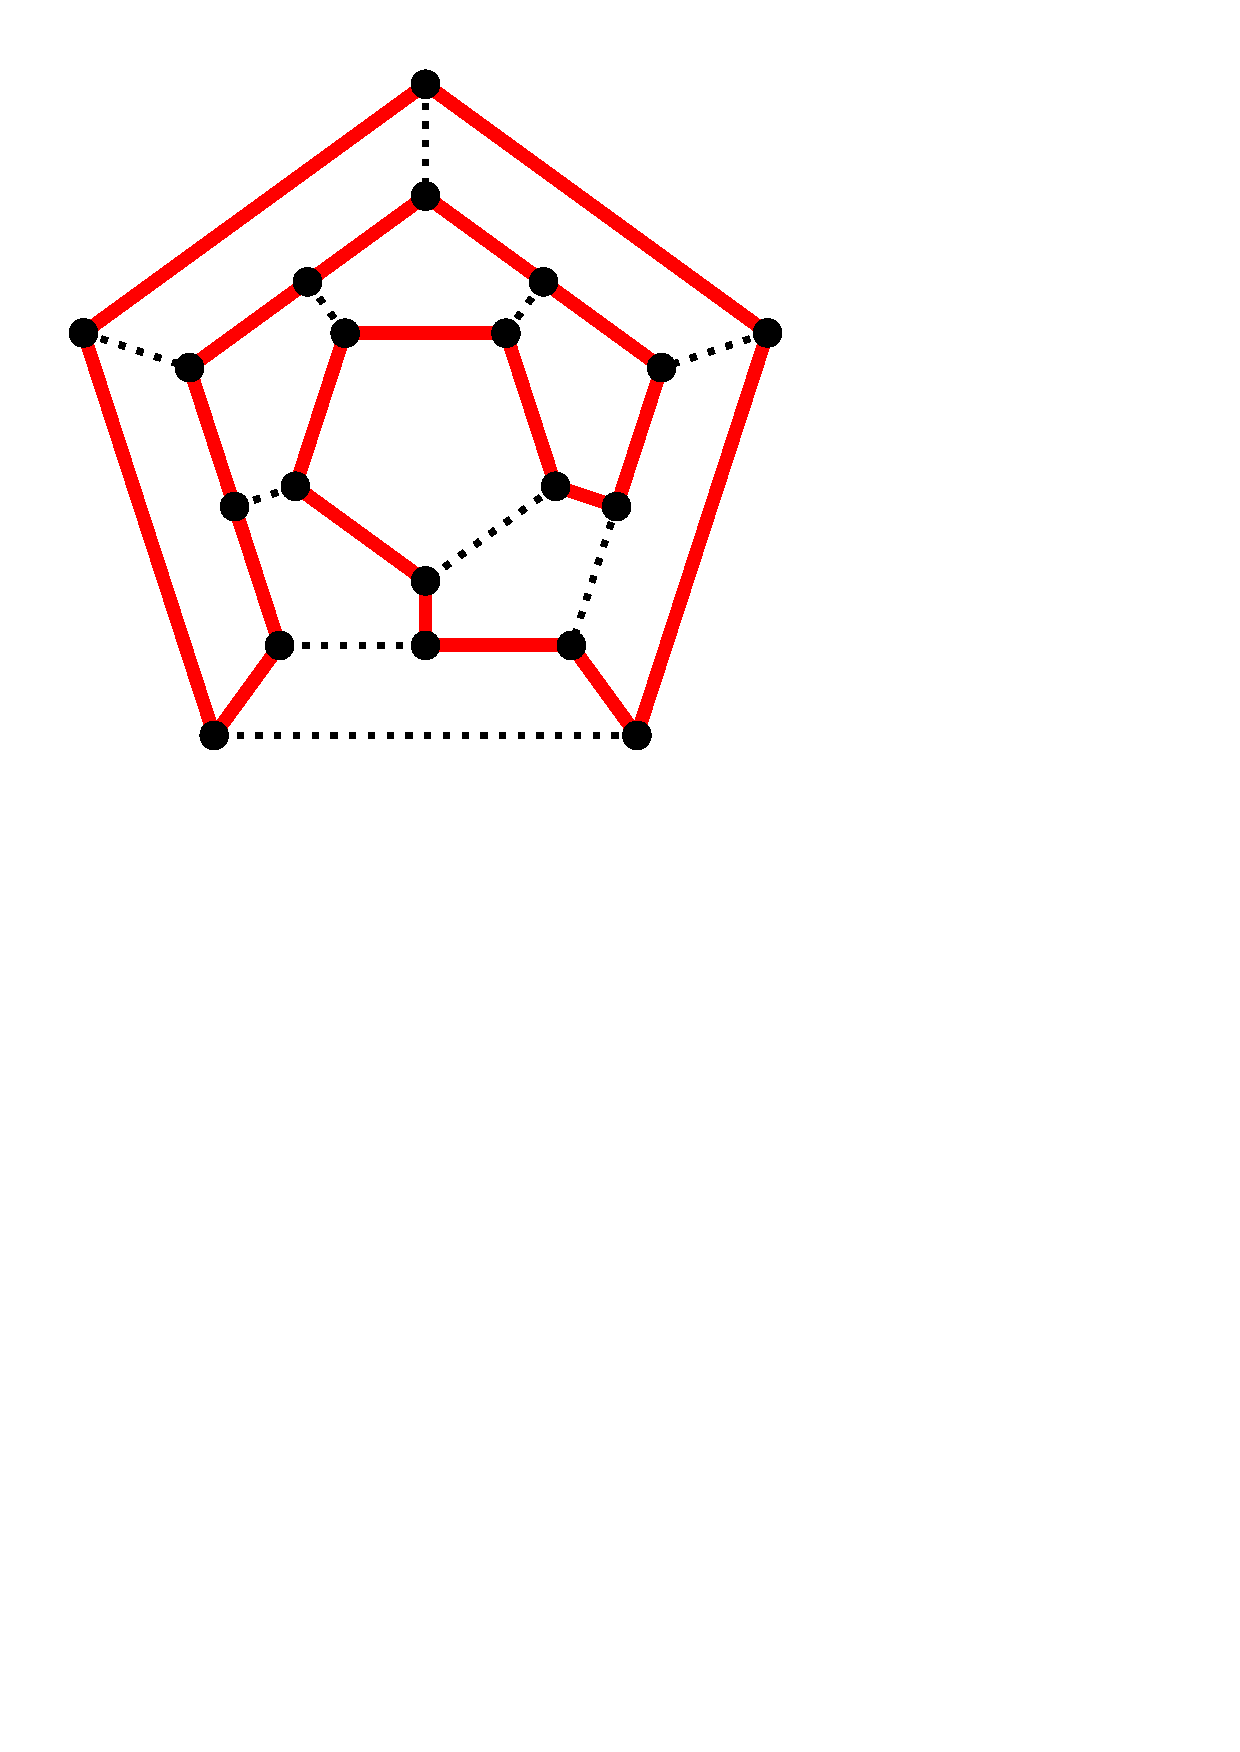
\includegraphics[width=0.8\textwidth]{hamiltonian-path}
\end{figure}
\end{minipage}

\subsubsection{La complessità si nasconde dove non te l'aspetti}

\paragraph{Circuito hamiltoniano}
Dato un grafo non orientato \(G\), esiste un circuito che attraversi ogni \emph{nodo} una e una sola volta?
\'E un problema {\NP}-completo.

\paragraph{Circuito euleriano}
Dato un grafo non orientato \(G\), esiste un circuito che attraversi ogni \emph{arco} una e una sola volta?
\'E un problema in {\PTIME}.

\paragraph{Cammini massimi}
Dato un grafo \(G = (V,E)\) e una funzione di peso \(w\) sugli archi, trovare il cammino con il peso \emph{massimo}.
\'E un problema {\NP}-completo.

\paragraph{Cammini minimi}
Dato un grafo \(G = (V,E)\) e una funzione di peso \(w\) sugli archi, trovare il cammino con peso \emph{minimo}.
\'E un problema in {\PTIME}.

\subsection{Problemi aperti}

\paragraph{Isomorfismo fra grafi}
Il problema dell’isomorfismo fra grafi richiede di determinare se due grafi finiti sono isomorfi.
Non sappiamo ancora se il problema sia {\NP}-completo o sia in {\PTIME}.
Il dibattito è ancora in corso.

\paragraph{Primalità}
Dato un numero \(n\), determinare se \(n\) è primo.
Questo problema è incluso in {\PTIME}.

\paragraph{Fattorizzazione}
Dato un numero \(n\), individuare i fattori primi che lo compongono.
Questo problema è sicuramente contenuto in {\NP}, si presume che non sia contenuto nè in {\PTIME}, nè che sia {\NP}-completo.

\subsubsection{Spunti di lettura}

Potete approfondire l'argomento nei seguenti testi:
\begin{itemize}
    \item Jeff Erickson, Algorithm. Cap. 12, NP-Hardness \href{http://jeffe.cs.illinois.edu/teaching/algorithms/}{http://jeffe.cs.illinois.edu/teaching/algorithms/};
    \item Sanjeev Arora, Boaz Barak. Computational complexity: a modern approach. Cambridge University Press, 2009. \href{http://theory.cs.princeton.edu/complexity/}{http://theory.cs.princeton.edu/complexity/}.
\end{itemize}

\begin{figure}[H]\centering
    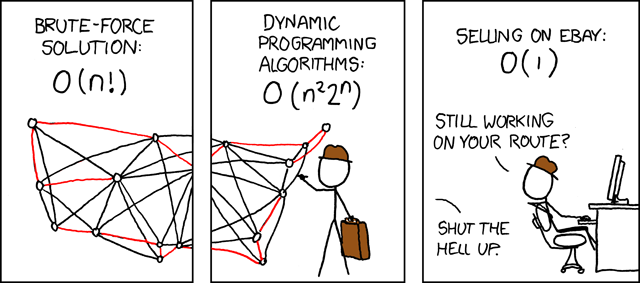
\includegraphics[width=0.6\textwidth]{tsp-xkcd}
\end{figure}

\ifsubfile
\end{document}
\fi
